\documentclass[10pt]{beamer}
\setbeamertemplate{navigation symbols}{}%remove navigation symbols
\usepackage{booktabs}
\usepackage{subfig}
\usepackage[newfloat]{minted}
\usepackage{listings}
\usepackage{lmodern}
\usepackage[T1]{fontenc}
\usefonttheme{professionalfonts}
%\usefonttheme{serif}
\usepackage{fontspec}
%\usepackage{kantlipsum}
\setbeamerfont{note page}{family*=pplx,size=\footnotesize}
\useoutertheme{infolines}
\usepackage[framemethod=tikz]{mdframed}
\usetikzlibrary{shadows}
\newmdenv[shadow=true,shadowcolor=black,font=\sffamily,rightmargin=8pt]{shadedbox}
\usepackage{pifont,xcolor}% http://ctan.org/pkg/{pifont,xcolor}
\definecolor{myblue}{RGB}{49,54,149}
\definecolor{myred}{RGB}{165,0,38}
\usepackage{graphicx}
\usepackage{caption}
\newcommand{\lenitem}[2][.55\linewidth]{\parbox[t]{#1}{#2\strut \strut}}

\usetheme{Frankfurt}

   \usefonttheme{professionalfonts} 
\newenvironment{variableblock}[3]{%
  \setbeamercolor{block body}{#2}
  \setbeamercolor{block title}{#3}
  \begin{block}{#1}}{\end{block}}
\usecolortheme{dove}
\usepackage{fancybox}
\setbeamercolor{block title}{bg=white,fg=black}
\newenvironment{fminipage}%
{\begin{Sbox}\begin{minipage}}%
{\end{minipage}\end{Sbox}\fbox{\TheSbox}}

\newcommand{\itemcolor}[1]{% Update list item colour
  \renewcommand{\makelabel}[1]{\color{#1}\hfil ##1}}

\newcounter{tmpc}
%\usefonttheme{structuresmallcapsserif}
\setbeamercolor{section in head/foot}{fg=black, bg=white}

\setbeamertemplate{frametitle}
{
    \nointerlineskip
    \begin{beamercolorbox}[sep=0.3cm,ht=1.8em,wd=\paperwidth]{frametitle}
        \vbox{}\vskip-3ex%
        \strut\insertframetitle\strut
        \vskip-1.2ex%
    \end{beamercolorbox}
}
\addtobeamertemplate{frametitle}{\vskip0.5ex}{}
\makeatletter
\setbeamertemplate{footline}
{
  \leavevmode%
  \hbox{%
  \begin{beamercolorbox}[wd=.875 \paperwidth,ht=2.25ex,dp=1ex,left]{section in head/foot}%
    \usebeamerfont{author in head/foot}\quad \quad \insertshorttitle
 \end{beamercolorbox}%
 \begin{beamercolorbox}[wd=.125\paperwidth,ht=2.25ex,dp=1ex,right]{section in head/foot}%
    \usebeamerfont{date in head/foot}\insertshortdate \quad \quad
    \insertframenumber{} / \inserttotalframenumber\hspace*{2ex} 
  \end{beamercolorbox}}%
  \vskip0pt%
}
\makeatother

\def\mf{
\begin{itemize}
\item Item
\end{itemize}
}
%\setbeamercolor{itemize item}{fg=yellow,bg=white}
%\setbeamertemplate{itemize items}[circle]
\setbeamercolor{enumerate item}{ fg=red}
\setbeamercolor{item projected}{bg=myblue}
\section{Title/Intro}
\subsection{Subsection}

\usepackage{listings}

\lstdefinestyle{BashInputStyle}{
  language=bash,
  basicstyle=\small\sffamily,
  numbers=left,
  numberstyle=\tiny,
  numbersep=5pt,
  framexleftmargin=3mm,
  frame=shadowbox, rulesepcolor=\color{gray},
  numberstyle=\normalfont\tiny\color{myred},
%  fillcolor=\color{gray},
  rulecolor=\color{black},
  columns=fullflexible,
  backgroundcolor=\color{white},
  linewidth=0.9\linewidth,
  xleftmargin=0.1\linewidth
}


\begin{document}
\small
\title{An Introduction to the Command Line Interface} 
\date{}
\author[Charles Rahal and Felix Tropf \\ Department of Sociology]{\includegraphics[width=0.225\textwidth]{ncrmlogo}\hspace{1.175in} \includegraphics[width=0.15\textwidth]{esrclogo}\vspace{0.2in} \\Charles Rahal and Felix Tropf \\ University of Oxford, Department of Sociology}
\frame{\titlepage 
\begin{center}
\vspace{-0.65in}
\texttt{26th June, 2017}\\ \vspace{0.2in}

\color{myblue}NCRM Summer School - University of Oxford\color{black}\\ \vspace{0.1in}
Slides, code, lecture notes: \color{myred}\url{https://github.com/crahal/Teaching}\color{black}\\ \vspace{0.1in}
Comments/questions/suggestions: \color{myred}\url{charles.rahal@sociology.ox.ac.uk}\\ \vspace{0.1in}
%Please note: if there is anyone here\color{red}\textbf{extremely preliminary}\color{black}.\\ \vspace{0.35in}
\end{center}
}


\subsection{}
\frame{
\frametitle{Some Class Administration}
\begin{itemize}
\item \textbf{WELCOME!} - to the NCRM Summer School in SocioGenomics! \pause \vspace{0.05in}
\item I'd like to also introduce \href{http://felix-tropf.com/}{\texttt{Felix}}: the TA for this class.\pause \vspace{0.05in}
\item This is the first of several computer workshops - each focusing on different things. \pause \vspace{0.05in}
\item Other classes are different, involving the practical use of the tools described here. \pause \vspace{0.05in}
\item From the pre-sessional materials, you should have set up a CLI:\vspace{0.05in}
\begin{itemize}
\item \textbf{Windows:} this will involve a VM. If you haven't managed this, I'll help you directly after this session or this evening before or after dinner.\vspace{0.05in}
\item \textbf{Linux or Mac:} you already have a command line -- nothing extra required. \pause \vspace{0.05in}
\end{itemize}
\item However: for a lot of classes, this isn't necessary, where a simple R (more often) or Python (less often) will be more than sufficient in your Windows environment. \pause \vspace{0.05in}
\item The CLI will only be required for some classes, but practicing with it this week provides \textbf{invaluable} experience for HPCs (an integral part of genomics).
\end{itemize}
}


\subsection{}
\frame{
\frametitle{Why Use the Command Line?}
Lets first further motivate \emph{why} we want to use the command line. Although there are many reasons for utilizing it, and conversely many reasons for maintaining a GUI for a lot of tasks, CLIs are important for these reasons especially:\vspace{0.1in}\pause
\begin{itemize}
\item Genetics datasets are \textbf{BIG}. The just released UK Biobank dataset is about 8tb. This necessitates the use of \textbf{H}igh \textbf{P}erformance \textbf{C}omputers (HPCs). The recent flood of genetic data is due to the reduced cost of genomic sequencing (specifically NGS) from around 2008.\vspace{0.1in}\pause
\item Automation/Replication:  No matter how complex the command or series of commands, the CLI doubles as a scripting language (shell scripts - which we will briefly discuss if there's time) which can be ran as a batch.\vspace{0.1in}\pause
\item Control: Commands are often more powerful and precise, giving more control over the operations to be performed\vspace{0.1in}\pause
\item Software tools: A number of genetics software tools will only run in Linux/Mac environments.  
\end{itemize}
}


\subsection{}
\frame{
\frametitle{Our Friend - ARCUS (or AWS)}
\begin{itemize}
\item Why have this class at all? Our friend ARCUS \href{http://www.arc.ox.ac.uk/content/introduction-linux}{\color{myred}provides some motivation}:\vspace{0.1in}
\begin{center}
   \includegraphics[width=0.9\textwidth]{figure1.png}
\end{center}
\pause
\item The CLI can seem like a harsh, unforgiving environment.\vspace{0.1in} \pause
\item \href{http://www.urbandictionary.com/define.php?term=rm\%20-rf\%20\ q\%2F}{\color{myred}Urban Dictionary} calls the famous CLI command \texttt{rm -rf}:
\begin{center}
 \emph{`the finest compression available under UNIX/Linux...\\ unfortunately, there is no decompresser available.'}\vspace{0.1in}\pause
 \end{center}
\item However: \textbf{the potential is endless!}\vspace{0.1in}\pause
\item (and a Virtual Machine is the best way to learn).
\end{itemize}
}

\subsection{}
\frame{
\frametitle{This isn't a scary course!}
\begin{itemize}
\item Melinda told me that a good strategy is to put a picture of your cat on the slides to persuade participants that the course isn't scary...  \pause
\end{itemize}
\begin{figure}[!b]
\centering  
\caption{This isn't a scary course!}\label{figure_5}
\subfloat[Sleepy]{\label{figure_5a}\includegraphics[width=0.35\textwidth]{moonpie1.png}}\hspace{0.4in}
\subfloat[Curious]{\label{figure_5b}\includegraphics[width=0.34\textwidth]{moonpie3.png}}\\
\normalsize
\end{figure}
%And now is probably the best time to do that.
}


\subsection{}
\frame{
\frametitle{A Brief History of nix*-like environments}
\begin{itemize}
\item Before we discuss \emph{exactly} what the CLI is, we should briefly talk about the history of what is now known as *nix-like computing.\vspace{0.1in}\pause
\item Unix was created 1969 at Bell Laboratories -- then a development division at AT\&T -- by Ken Thompson and Dennis Richie.\vspace{0.1in}\pause
\item All software previously hardware dependent, written in assembler language.\vspace{0.1in}\pause
\item However -- a critical feature of Unix was that it is proprietary.\vspace{0.1in}\pause
\item University of California, Berkley developed BSD -- based on the AT\&T code base. Commercial Unix derivatives emerged through the 1980s (i.e. Mac OS).\vspace{0.1in}\pause
\item The breakthrough came in September 1991, when Linus Torvalds released the Linux operating system kernel.\vspace{0.1in}\pause
\item \textbf{Utilized everywhere:} i.e. Android operating system and Chrome OS which runs on Chromebooks (televisions,  smart-watches, servers, etc).\vspace{0.1in}
\end{itemize}
}

\subsection{}
\frame{
\frametitle{The File Tree}
\vspace{-.3in}
\begin{center}
   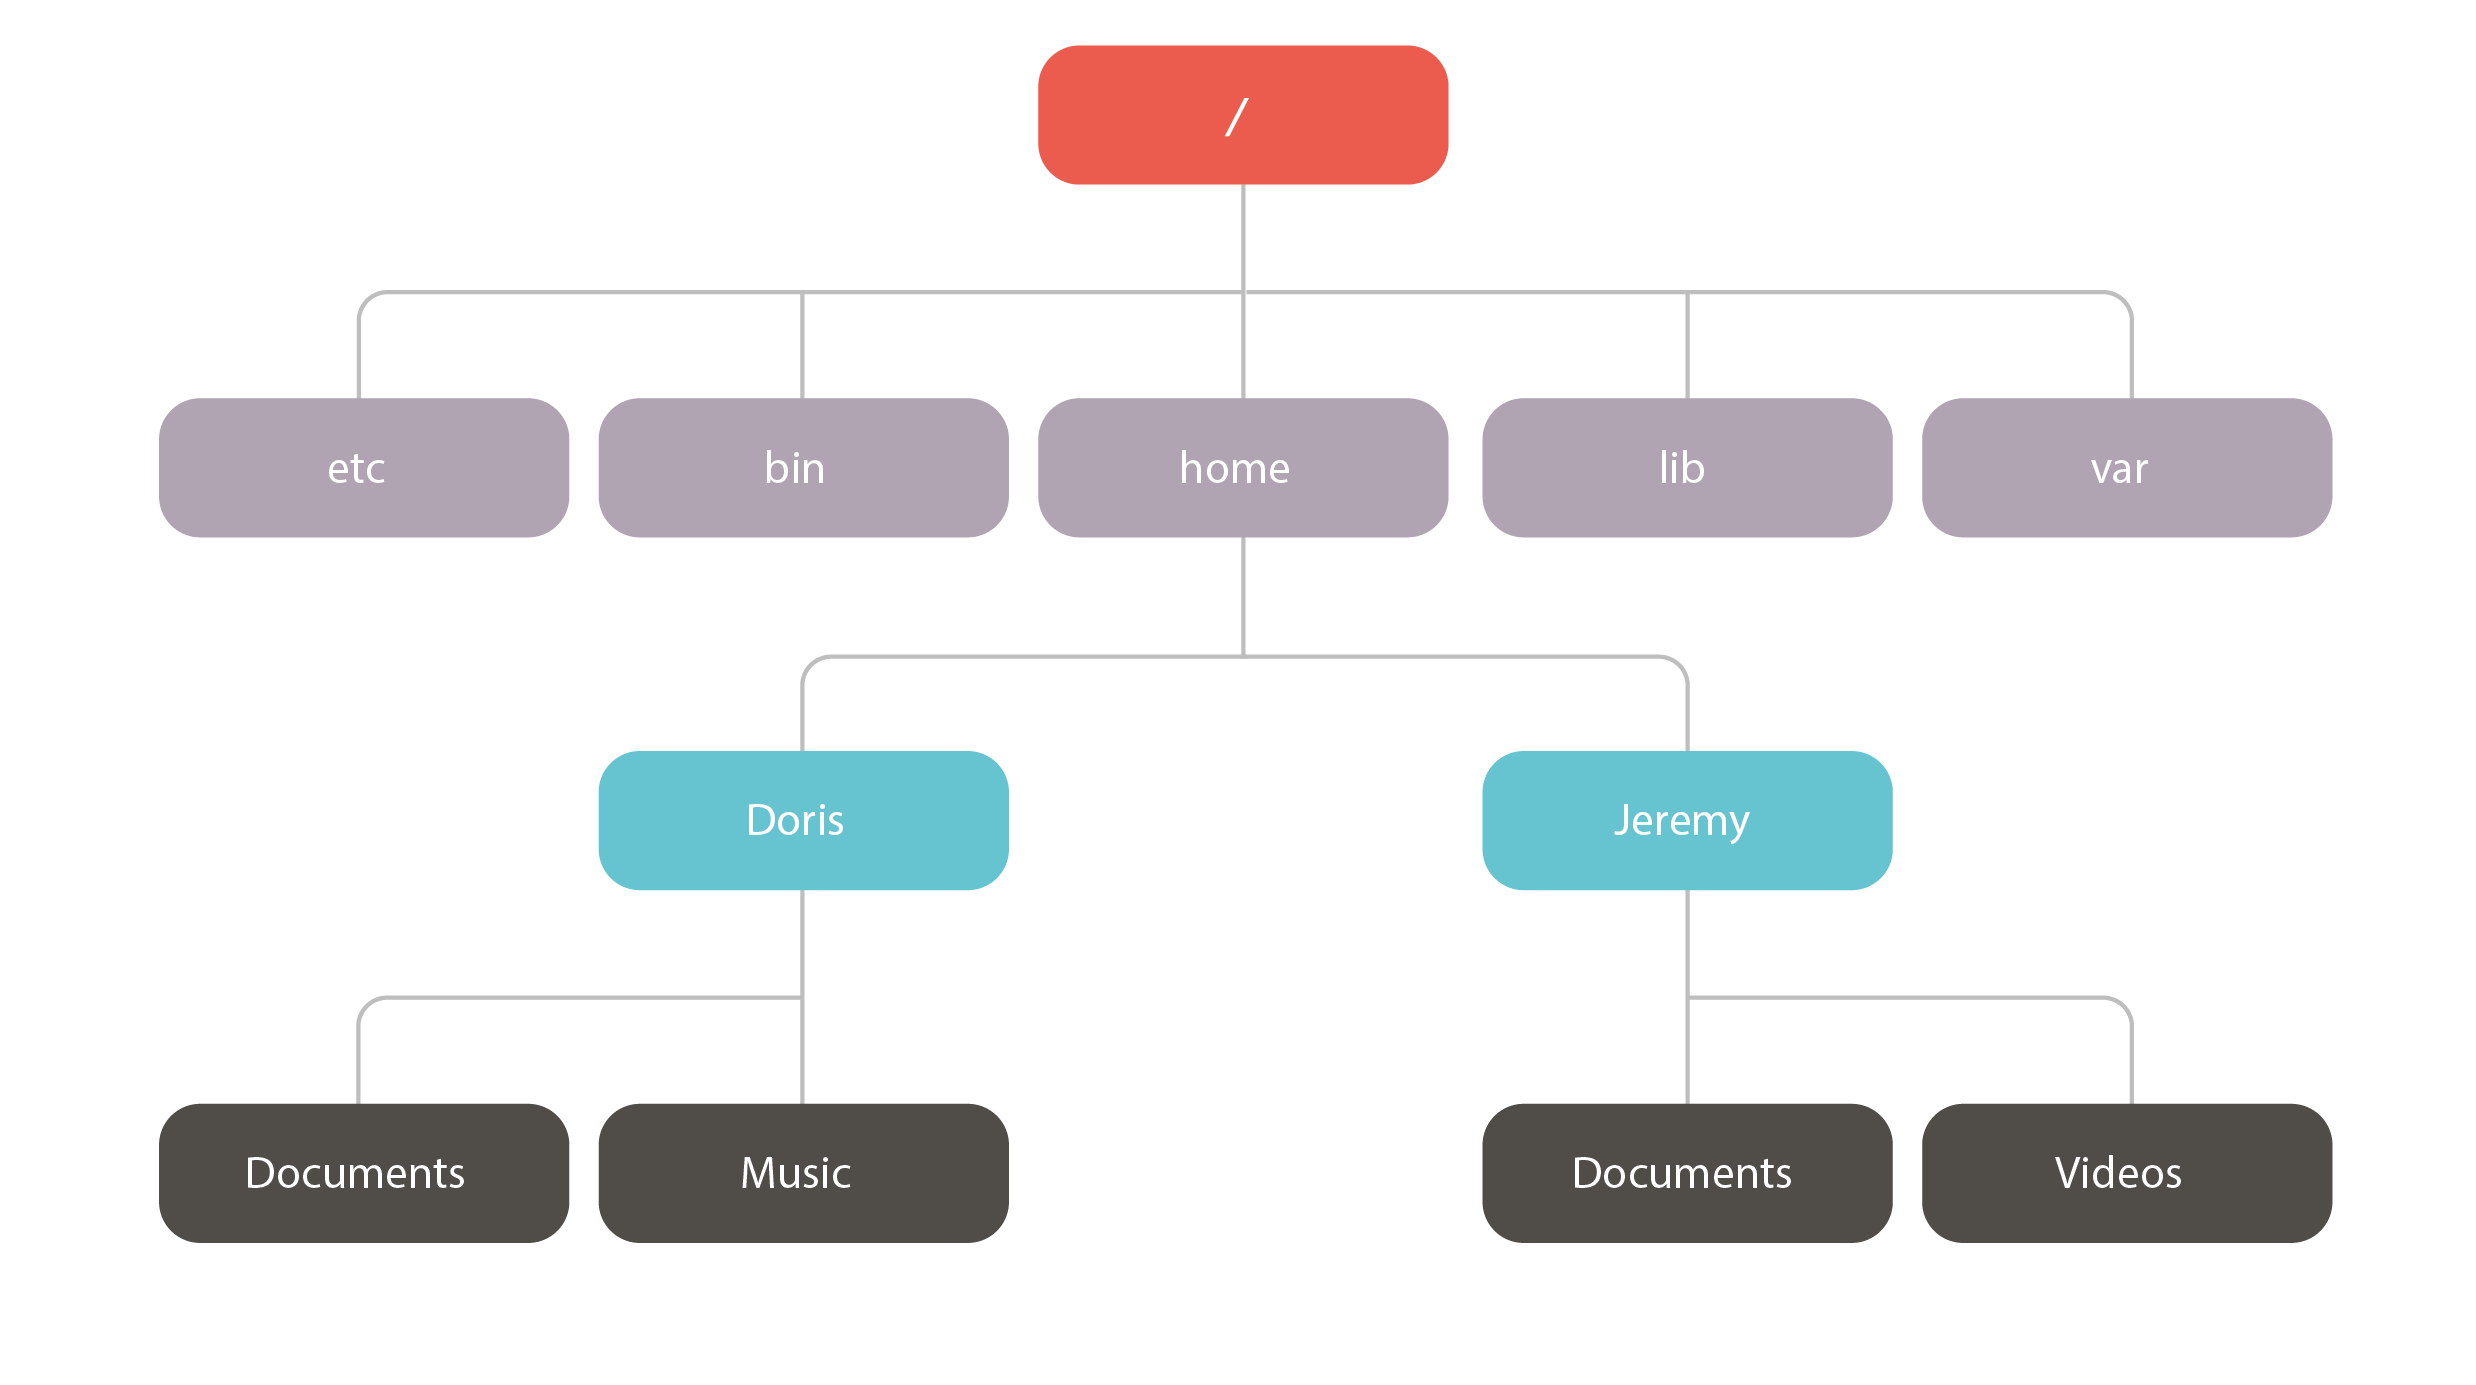
\includegraphics[width=0.85\textwidth]{Infographic2.png}
\end{center}
\
\begin{itemize}
\item You might also find  \texttt{/opt:} optional software or \texttt{/tmp:} temporary space.
\end{itemize}
}

\subsection{}
\frame{
\frametitle{System Architecture}
\begin{center}
   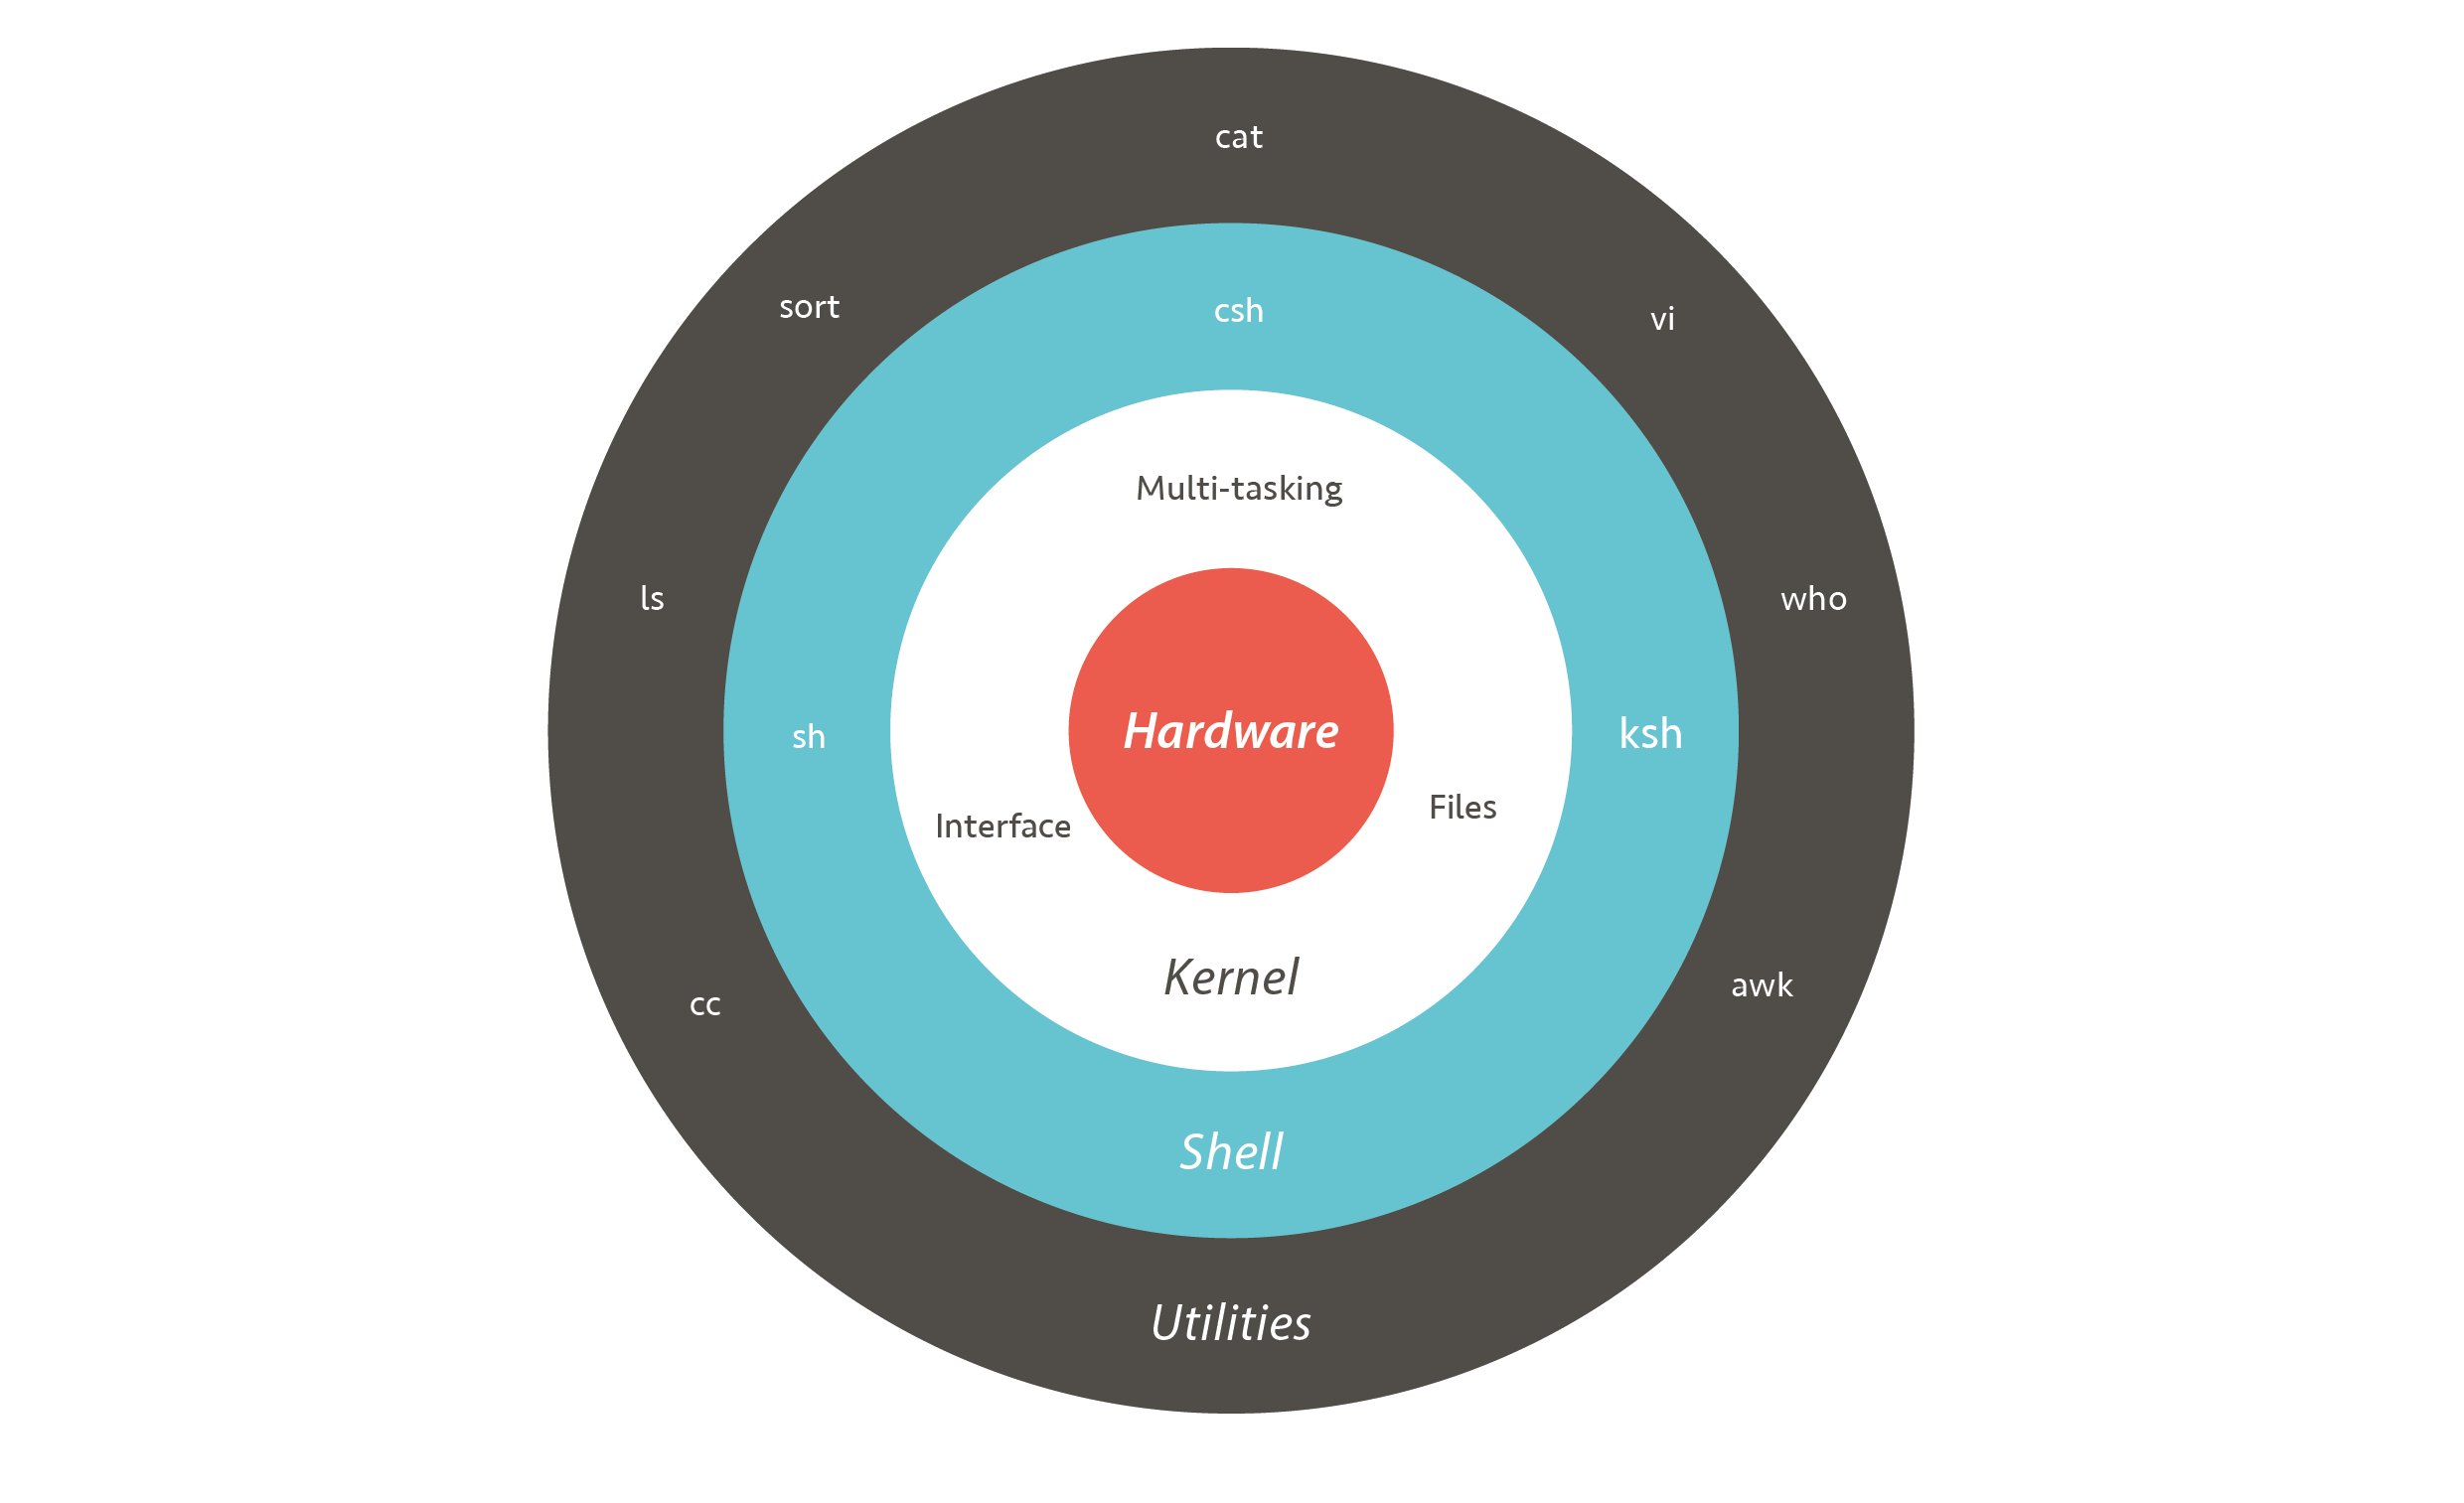
\includegraphics[width=0.7\textwidth]{Infographic1.png}
\end{center}
\begin{itemize}
\item The shell is a friendly interface that translates your commands into some low-level calls to the kernel.
\end{itemize}
}

\subsection{}
\frame{
\frametitle{The Terminal}
\begin{itemize}
\item The terminal is a program which lets you interact with the shell:\vspace{0.1in}
\end{itemize}
\begin{center}
   \includegraphics[width=0.75\textwidth]{theterminal.png}
\end{center}
\begin{itemize}
\item If the last character of your shell prompt is \# rather than \$, you are operating as the superuser. This means that you have administrative privileges. This can be potentially dangerous, since you are able to delete or overwrite any file on the system. Unless you absolutely need administrative privileges, do not operate as the superuser (try \texttt{whoami} and \texttt{sudo whoami}).
\end{itemize}
}

\section{Fundamental Commands}
\subsection{}
\begin{frame}[fragile]{Examples}
\frametitle{Fundamental CLI Commands: \texttt{man}}
\begin{itemize}
\item The \texttt{man} command shows the manual for a given page, including information on options and usage.\vspace{0.1in}
\item This is the default resource for getting help on specific commands.\vspace{0.1in}
\begin{lstlisting}[style=BashInputStyle, title=The \texttt{man} Command]
user@system:~$ man echo
ECHO(1)                  User Commands                 ECHO(1)

NAME
       echo - display a line of text

SYNOPSIS
...
\end{lstlisting}
\item For example, the \texttt{man echo} command will display the manual for the \texttt{echo} command which we just saw.\\
\end{itemize}
\end{frame}


\subsection{}
\begin{frame}[fragile]{Examples}
\frametitle{Fundamental CLI Commands: \texttt{whatis}}
\begin{itemize}
\item The \texttt{whatis} command gives a short summary description of the specific command, and command inputs can be stacked together. \vspace{0.2in}
\begin{lstlisting}[style=BashInputStyle,title=The \texttt{whatis} Command]
user@system:~$ whatis echo ls
echo (1)             - display a line of text
ls (1)               - list directory contents
\end{lstlisting}
\vspace{0.1in}
\item Each manual page has a short description available within it -- and \texttt{whatis} searches the manual page names.
\end{itemize}
\end{frame}




\subsection{}
\begin{frame}[fragile]{Examples}
\frametitle{Fundamental CLI Commands: \texttt{ls}}
\begin{itemize}
\item \texttt{ls} is a Linux shell command that lists directory contents of files and directories.\vspace{0.2in}
\end{itemize}
\begin{lstlisting}[style=BashInputStyle,title=The \texttt{ls} Command]
user@system:~$ ls
Desktop Documents Downloads Music Pictures Public Videos
\end{lstlisting}
\vspace{0.1in}
\begin{itemize}
\item The lists can also be sorted, accept wildcards, and pipe outputs to file. \vspace{0.1in}
\item It can show hidden files, show file size, and has the option for a `long' format.\vspace{0.1in}
\end{itemize}
\end{frame}

\subsection{}
\begin{frame}[fragile]{Examples}
\frametitle{Fundamental CLI Commands: \texttt{pwd}}
\begin{itemize}
\item However, this isn't much use without knowing \emph{where} we are in the file tree. \vspace{0.2in}
\end{itemize}
\begin{lstlisting}[style=BashInputStyle,title=The \texttt{pwd} Command]
user@system:~$ pwd
/home/user
\end{lstlisting}
\vspace{0.1in}
\begin{itemize}
\item In *nix-like operating systems, the \texttt{pwd} command (which stands for print working directory) writes the full path-name of the current working directory to the standard output.\\
\end{itemize}
\end{frame}

\subsection{}
\begin{frame}[fragile]{Examples}
\frametitle{Fundamental CLI Commands: \texttt{mkdir} and \texttt{cd}}
\begin{itemize}
\item We should make a new directory for the summer school. \vspace{0.05in}
\end{itemize}
\begin{lstlisting}[style=BashInputStyle,,title=The \texttt{mkdir} and \texttt{cd} Commands]
user@system:~$ mkdir NCRM
user@system:~$ ls
NCRMTextbookChapter
user@system:~$ cd NCRM
user@system:~/NCRM$ pwd
/home/user/NCRM
\end{lstlisting}
\vspace{0.1in}
\begin{itemize} 
\item This brings us to the concept of \emph{absolute} and \emph{relative} paths. \vspace{0.05in}
\item From the documents folder above, we can navigate to the new folder (\texttt{NCRM}) through the relative path or through the absolute path. \vspace{0.05in}
\item The \texttt{cd} command is used to change the current directory.\vspace{0.05in}
\item There are multiple ways of identifying the same file path in the directory tree.
\end{itemize}
\end{frame}

\subsection{}
\begin{frame}[fragile]{Examples}
\frametitle{Fundamental CLI Commands: \texttt{touch}}
\begin{itemize}
\item The \texttt{touch} command is the easiest way to create new, empty files...
\end{itemize}
\begin{lstlisting}[style=BashInputStyle,title=The \texttt{touch} Command]
user@system:~/NCRM$ touch testfile
user@system:~/NCRM$ ls
testfile
\end{lstlisting}
\vspace{0.1in}
\begin{itemize}
\item \texttt{testfile} might seem unfamiliar to you for one obvious reason: the lack of an extension. \vspace{0.1in}
\item  In *nix-like systems, the extension is ignored, and the file type is determined automatically (and the command \texttt{file} can tell us additional information).\vspace{0.1in}
\end{itemize}
\end{frame}

\subsection{}
\begin{frame}[fragile]{Examples}
\frametitle{Fundamental CLI Commands: \texttt{rm}}
\begin{itemize}
\item Now that we can create files and directories, lets look at removing them:
\end{itemize}
\begin{lstlisting}[style=BashInputStyle,title=The \texttt{rm} Command]
user@system:~/NCRM$ cd ..
user@system:~/$ rm -ri NCRM
rm: remove directory 'NCRM'?
\end{lstlisting}
\vspace{0.1in}
\begin{itemize}
\item This shows how we can stack options together, where \texttt{rm -ri} is the equivalent to \texttt{rm -r -i}. \vspace{0.05in}
\item However, command line options are not universal between commands, and implementation across different operating systems may vary.\vspace{0.05in}
\item We should also note the existence of \texttt{rmdir}, the negative equivalent to \texttt{mkdir}, which removes \emph{empty} directories. \vspace{0.05in}
\item Note the use of \texttt{..} to move up a directory (and many other similar shortcuts).
\end{itemize}
\end{frame}

\subsection{}
\begin{frame}[fragile]{Examples}
\frametitle{Fundamental CLI Commands: \texttt{mv} and \texttt{cp}}
\begin{itemize}
\item It seems only natural that we now learn how to move, copy and rename files.
\end{itemize}
\begin{lstlisting}[style=BashInputStyle,title=The \texttt{mv} and \texttt{cp} Commands]
user@system:~/NCRM$ cp testfile ..
user@system:~/NCRM$ rm ../testfile
user@system:~/NCRM$ mv testfile ..
\end{lstlisting}
\vspace{0.1in}
\begin{itemize}
\item We need not actually remove \texttt{testfile} after copying it and before moving it, as the \texttt{mv} command would simply overwrite it.\vspace{0.1in}
\item To rename a file, we can just move it with a new name. 
\end{itemize}
\end{frame}

\subsection{}
\begin{frame}[fragile]{Examples}
\frametitle{Other Basic Utilities}
\begin{itemize}
\item We can \texttt{clear} the terminal screen.\vspace{0.1in}
\item We can display all environmental variables with \texttt{env} (try \texttt{echo \$LANG}).\vspace{0.1in}
\item \texttt{find} and \texttt{locate} search for files and directories (with the latter being faster -- performing on a database of indexed filenames).\vspace{0.1in}
\item  \texttt{date} displays or sets (with the option \texttt{-s}) the system time, and \texttt{cal} displays the calender.\vspace{0.1in}
\item \texttt{history} and specifically - \texttt{history [NUM]} reports the last \texttt{[NUM]} commands.\vspace{0.1in}
\item We can \texttt{exit} from the current terminal session, \texttt{logout} as a specific user, or \texttt{shutdown} the machine entirely.\vspace{0.1in}
\item We can also \texttt{tar} items together, and then \texttt{gzip} or \texttt{bzip2} them up.
\end{itemize}
\end{frame}

\section{More Advanced Concepts}
\subsection{}
\begin{frame}[fragile]{Examples}
\frametitle{Editors at the Command Line}
\begin{itemize}
\item Lets introduce the use of text editors at the command line (vi, pico, nano and emacs). These are plain text editors -- not word processing suites.\vspace{0.1in}
\item Unlike many GUI based editors, the mouse does not move the cursor. Unlike PC editors, you cannot modify text by highlighting it with a mouse.\vspace{0.1in}
\item Lets use \texttt{nano} to create a file which we will use for some examples later on: a list of all the fruits we can think of (call the file \texttt{allfruits}). \vspace{0.1in}
\end{itemize}
\begin{lstlisting}[style=BashInputStyle,title=Introducing Text Editors at the CLI: \texttt{nano allfruits}]
Apple
Apricot
Avocado
.
.
"allfruits" 90 lines, 846 characters
\end{lstlisting}
\end{frame}

\subsection{}
\begin{frame}[fragile]{Examples}
\frametitle{I/O Redirection}
\begin{itemize}
\item Most command line programs output their results to the ‘standard output’ (STDOUT): which, by default, is the display.
\item We can redirect standard output to specific files using the ‘>’ character, and append to a file using ‘> >’.
\item Commands can also accept input from ‘standard input’ (STDIN), which defaults to the keyboard: to redirect from STDIN, we use the ‘<’ character.
\end{itemize}
\begin{lstlisting}[style=BashInputStyle,title=STDOUT and STDIN]
user@system:~/NCRM$ ls > filelist.txt
user@system:~/NCRM$ sort < filelist.txt
\end{lstlisting}
\begin{itemize}
\item There is also a third stream which will go unexamined (‘standard error’ or STDERR) which is used for error messages – and also defaults to the terminal.
\end{itemize}
\end{frame}

\subsection{}
\begin{frame}[fragile]{Examples}
\frametitle{Filters}
\emph{filters} are a class of programs which are extremely useful for I/O Redirection:\vspace{0.1in}
\begin{itemize} 
\item \texttt{sort:} Sorts STDIN and outputs the sorted result on standard output.\vspace{0.05in}
\item \texttt{uniq}: Given a sorted stream of data from STDIN, it removes duplicates.\vspace{0.05in}
\item \texttt{head}: Outputs the first few lines of its input (defaults to first 10 lines).\vspace{0.05in}
\item \texttt{cat}: Concatenates files and displays their contents, or just displays contents if given one input.\vspace{0.05in}
\item \texttt{less}: used to view (but not change) the contents of a text file one screen at a time.\vspace{0.05in}
\item \texttt{cut}: Divides a file into several columns.\vspace{0.05in}
\item \texttt{nl}: prints the line number before data.\vspace{0.05in}
\item \texttt{wc}: which prints the count of lines, words and characters.\vspace{0.05in}
\end{itemize}
\end{frame}


\subsection{}
\begin{frame}[fragile]{Examples}
\frametitle{The Pipe}
\begin{itemize}
\item The pipe (\texttt{|}), which allows you to connect multiple commands together.\vspace{0.1in}
\item The standard output of one command is fed into the standard input of another, enabling you to chain together individual commands to create something really powerful.\vspace{0.1in}
\item The example below \emph{pipes} the output from \texttt{ls} into the \texttt{head} command which takes the input \texttt{1} to show us the first 1 line of the \texttt{ls} output: we've chained the two commands together.
\end{itemize}
\begin{lstlisting}[style=BashInputStyle, title=The Pipe \texttt{(|)}]
user@system:~/NCRM$ ls | head -1
allfruits
\end{lstlisting}
\end{frame}

\subsection{}
\begin{frame}[fragile]{Examples}
\frametitle{Wildcards}
\begin{itemize}
\item Another more advanced concept is the `wildcard': a set of tools that allow you to create a pattern which defines a specific set of files or directories.\vspace{0.1in}
\item There are two simple types of wildcards: 
\setbeamertemplate{enumerate items}[default]
\begin{enumerate}
\item \texttt{*} represents zero or more characters
\item \texttt{?} represents a single character.
\end{enumerate}
\begin{lstlisting}[style=BashInputStyle, title=Wildcards: \texttt{*} and \texttt{?}]
user@system:~/NCRM$ touch fileonea fileoneb filetwoa filetwob
user@system:~/NCRM$ ls file*a
fileonea filetwoa
user@system:~/NCRM$ ls filetwo?
filetwoa filetwob
\end{lstlisting}
\item A regular expression (or `regex') includes such functionality, but is a much more powerful pattern matcher beyond the scope of this introduction.
\end{itemize}
\end{frame}


\subsection{}
\begin{frame}[fragile]{Examples}
\frametitle{Grep}
\begin{itemize} 
\item One particularly useful filter is \texttt{grep}, which examines each line of data it receives from standard input and outputs every line that contains a specified pattern of characters.\vspace{0.05in}
\item It utility filters input, looking for matches.\vspace{0.05in}
\item Lets use it to find all examples of berries within our fruits file.\vspace{0.05in}
\item In our example, we pass it the -E option, which allows it to interpret the wildcard:\vspace{0.05in}
\begin{lstlisting}[style=BashInputStyle, title=The \texttt{grep} Command]
user@system:~/NCRM$ grep -E *berry allfruits
strawberry
raspberry
blackberry
\end{lstlisting}
\end{itemize}
\end{frame}


\subsection{}
\begin{frame}[fragile]{Examples}
\frametitle{Users, Groups and Permissions}
\begin{itemize}
\item Permissions  specify what a user can and cannot do: i.e. lock your files so other people cannot change them or secure system files from damage. \vspace{0.05in}
\item Permissions are split into three distinct categories which govern the ability to: Read: \texttt{r}, Write: \texttt{w} and Execute: \texttt{x}.\vspace{0.05in}
\item For every file, we need to define permissions for potential users: 
\begin{itemize}
\item The user who created the file (u).
\item The group which owns the file (g).
\item Others (o).\vspace{0.05in}
\end{itemize}
\item There are typically only two people who can manage the permissions of a given file or directory: the owner and the root user. \vspace{0.05in}
\item To view the permissions associated with an individual file, we can use the \texttt{-l} option on the \texttt{ls} command:\\ \vspace{0.05in}
\begin{lstlisting}[style=BashInputStyle]
user@system:~/NCRM$ ls -l allfruits
-rw-rw-r-- 1 user user 846 May 29 14:57 allfruits
\end{lstlisting}
\end{itemize}
\end{frame}

\subsection{}
\begin{frame}[fragile]{Examples}
\frametitle{Users, Groups and Permissions (Cont.)}
\begin{itemize}
\item The first character determines whether it is a file (\texttt{-}) or a directory (\texttt{d}).\vspace{0.05in}
\item We have information on the permissions for \texttt{u}, \texttt{g} and \texttt{o}.\vspace{0.05in}
\item A \texttt{-} represents the omission of a permission.\vspace{0.05in}
\item Change permissions with \texttt{chmod}, specifying: 1.) Who? 2.) Giving (\texttt{+}) or taking (\texttt{-})?, 3.) Which permissions\vspace{0.05in}
\item For example, lets take away read permissions from the group and others:
\begin{lstlisting}[style=BashInputStyle, title=The \texttt{chmod} Command]
user@system:~/NCRM$ chmod og-r allfruits
user@system:~/NCRM$ ls -l allfruits
-rw------- 1 user user 846 May 29 15:09 allfruits
\end{lstlisting}\vspace{0.05in}
\item Permissions are not inherited from the parent directory (unless \texttt{-R}: recursive).\vspace{0.05in}
\item There are a range of `short-hand' commands (e.g. \texttt{chmod 751 <filename>}).
\end{itemize}
\end{frame}

%\subsection{}
%\begin{frame}[fragile]{Examples}
%\frametitle{Archiving}
%\begin{itemize}
%\item Archiving in our context is similar to the familiar .zip extension in Windows. \vspace{0.05in}
%\item Introducing the tape archive -- \texttt{tar}: extract with \texttt{-x}, create with \texttt{-c.}.\vspace{0.05in}
%\item Typically compressed with \texttt{gzip} (Lempel-Ziv) or \texttt{bzip2} (Burrows-Wheeler).\vspace{0.05in}
%\end{itemize}
%\begin{lstlisting}[style=BashInputStyle]
%user@system:~/NCRM$ head -5 allfruits > top5fruits
%user@system:~/NCRM$ ls -la
%-rw------- 1 user user  846 May 30 13:32 allfruits
%-rw-rw-r-- 1 user user   38 May 30 13:33 first5fruits
%user@system:~/NCRM$ tar -cvf fruits.tar allfruits first5fruits
%user@system:~/NCRM$ gzip fruits.tar
%user@system:~/NCRM$ tar -cvf fruits.tar allfruits first5fruits
%user@system:~/NCRM$ bzip2 fruits.tar
%user@system:~NCRM$ bzip2 ls -l
%-rw------- 1 user user 10240 May 30 14:07 allfruits
%-rw-rw-r-- 1 user user    38 May 30 13:33 first5fruits
%-rw-rw-r-- 1 user user   214 May 30 14:13 fruitlists.tar.bz2
%-rw-rw-r-- 1 user user   224 May 30 14:13 fruitlists.tar.gz
%\end{lstlisting}\vspace{0.05in}
%\end{frame}

\section{Scripting}
\subsection{}
\begin{frame}[fragile]{Examples}
\frametitle{Bash Scripting: Introduction}
\begin{itemize}
\item Bash scripting performs complex, repetitive tasks with minimal effort.\vspace{0.05in}
\item A script is just a text file containing commands which could be ran directly.\vspace{0.05in}
\item It is a convention (albeit unnecessary) to give bash scripts an extension of .sh.
\end{itemize}
\begin{lstlisting}[style=BashInputStyle,title=Our first script: \texttt{myfirstscript.sh}]
#!/bin/bash
echo Hello There! Welcome to Bash Scripting!
\end{lstlisting}\vspace{0.05in}
\begin{itemize}
\item The first line is called the `shebang'. We can run the file in two ways:
\end{itemize}
\begin{lstlisting}[style=BashInputStyle,title=Executing \texttt{myfirstscript.sh}]
user@system:~/NCRM$ ./myfirstscript.sh
Hello There! Welcome to Bash Scripting!
user@system:~/NCRM$ bash myfirstscript.sh
Hello There! Welcome to Bash Scripting!
\end{lstlisting}
\end{frame}



\subsection{}
\begin{frame}[fragile]{Examples}
\frametitle{Bash Scripting: Variables}
\begin{itemize}
\item Just like in other languages: variables are temporary methods of storing information.\vspace{0.05in}
\item Setting them requires no \$, but reading them does.\vspace{0.05in}
\item Lets pass variables to a script which accepts \$1 and \$2 as inputs:\vspace{0.05in}
\end{itemize}
\begin{lstlisting}[style=BashInputStyle,title=Accepting Variables: \texttt{mysecondscript.sh}]
#!/bin/bash
echo Hello $1! Message sent from $2!
\end{lstlisting}\vspace{0.05in}
\quad and then execute it as before:\vspace{0.05in}
\begin{lstlisting}[style=BashInputStyle,title=Executing \texttt{mysecondscript.sh}]
user@system:~/NCRM$ ./variables.sh Felix Charlie
Hello Felix! Message sent from Charlie!
\end{lstlisting}\vspace{0.05in}
\begin{itemize}
\item There are also a number of special variables: \texttt{\$0}, \texttt{\$n}, \texttt{\$?} etc.
\end{itemize}
\end{frame}

\subsection{}
\begin{frame}[fragile]{Examples}
\frametitle{Bash Scripting: User Input}
\begin{itemize}
\item We can also ask the user for input using \texttt{read}:
\end{itemize}
\begin{lstlisting}[style=BashInputStyle,title=Asking for User Input: \texttt{mythirdscript.sh}]
#!/bin/bash
echo Hey, Buddy! What is your favorite color?
read favoritecolor
echo Wow! $favoritecolor is my favorite color too!
\end{lstlisting}\vspace{0.1in}
\quad and then execute it as before:\vspace{0.1in}
\begin{lstlisting}[style=BashInputStyle,title=Executing \texttt{mythirdscript.sh}]
user@system:~/NCRM$ ./readvariable.sh
Hey, Buddy! What is your favorite color?
Blue
Wow! Blue is my favorite color too!
\end{lstlisting}\vspace{0.1in}
\end{frame}

\subsection{}
\begin{frame}[fragile]{Examples}
\frametitle{Bash Scripting: Arithmetic}
\begin{itemize}
\item Do simple arithmetic operations with \texttt{let} (store) and \texttt{expr} (print). We can utilize the standard operators of \textbf{+}, \textbf{-}, \textbf{$\backslash$*},\textbf{ /}.
\end{itemize}
\begin{lstlisting}[style=BashInputStyle,title=Simple Arithmetic Operations: \texttt{myfourthscript.sh}]
#!/bin/bash
let ``a = $1 + $2''
echo adding $1 and $2 together gives $a
echo multiplying $1 and $2 together gives $(expr $1 \* $2)
\end{lstlisting}\vspace{0.05in}
\quad and then execute it as before:
\begin{lstlisting}[style=BashInputStyle,title=Executing \texttt{myfourthscript.sh}]
user@system:~/NCRM$ ./arithmetic.sh 10 5
adding 10 and 5 together gives 15
multiplying 10 and 5 together gives 50
\end{lstlisting}\vspace{0.05in}
\begin{itemize}
\item Finally, we can also embed \texttt{if} statements just like in other languages (no indentation), and utilize various types of loops (while, until and for).\vspace{0.05in}
\end{itemize}
\end{frame}

\section{Python and R}
\subsection{}
\begin{frame}[fragile]{Examples}
\frametitle{Python and R}
\begin{itemize}
\item HPCs requires us to submit our Python and R scripts through the CLI.\vspace{0.05in}
\item This is as simple as writing your R or Python scripts locally and then transferring them (\texttt{scp} or \texttt{rsync}) or writing them using a CLI editor.\vspace{0.05in}
\item Lets create an example file called \texttt{helloworld} which simply has the single line: \texttt{print(''Hello World! How are you?'')}.\vspace{0.05in}
\item Assuming Py 2, we can execute \texttt{helloworld} with almost identical output:\vspace{0.05in}
\begin{lstlisting}[style=BashInputStyle,title=Executing Python and R Scripts in the CLI]
user@system:~/NCRM$ python helloworld
Hello World! How are you?
user@system:~/NCRM$ Rscript helloworld
[1] ``Hello World! How are you?''
\end{lstlisting}\vspace{0.1in}
\item We can execute the files with \texttt{./} as above, but this requires a \texttt{shebang}! \#!/usr/bin/Rscript for R and \#!/usr/bin/env python. 
\end{itemize}
\end{frame}


\section{Conclusion}
\subsection{}
\begin{frame}[fragile]{Examples}
\frametitle{Conclusion}
\begin{itemize}
\item We've gone through the main basic ideas behind the CLI, with the intention of providing some intuition.\vspace{0.05in}\pause
\item Other courses use these ideas in their application to sociogenomics.\vspace{0.05in}\pause
\item We didn't really cover: alias-ing, networking, \textbf{ssh-ing}, scheduling, \texttt{awk} or \texttt{sed}, and we didn't fully consider control statements, or regex.\vspace{0.05in} \pause
\item Hopefully you now feel as suave with the CLI as this guy:
\end{itemize}
\begin{figure}[!b]
\includegraphics[width=0.4\linewidth]{clevercat.jpg}
\end{figure}
\end{frame}

\end{document}